\begin{frame}{3.3: executive summary}
\alert{Definitions:} orthogonality, orthogonal projection (onto vector and onto plane), point-normal form of lines and planes. 
\bspace
\alert{Procedures:} finding orthogonal projections onto lines and planes, finding distance between point and line, point and plane. 
\bspace
\alert{Theorems:} Pythagorean theorem for orthogonal vectors in $\R^n$. 
\end{frame}
\begin{frame}{3.3: orthogonality, lines and planes}
\footnotesize
\begin{definition}
Two vectors $\boldv,\boldw\in\R^n$ are {\bf orthogonal} if $\boldv\cdot\boldw=0$. We write $\boldv \perp \boldw$ in this case. 

This is equivalent to the angle $\theta$ between $\boldv$ and $\boldw$ being $\pi/2$ (or $90^\circ$). 
\end{definition}
\bpause 
Note that by definition it is very easy to check: $\boldv\perp\boldw$ iff $\boldv\cdot\boldw=0$. As a first simple example of the usefulness of orthogonality, we prove the following generalization of the Pythagorean Theorem. 
\begin{theorem}
Let $\boldv,\boldw\in\R^n$, and suppose  $\boldv\perp\boldw$. Then 
\[
\norm{\boldv}^2+\norm{\boldw}^2=\norm{\boldv+\boldw}^2.
\]
\end{theorem}
\pause
\begin{proof}
\begin{eqnarray*}
\norm{\boldv+\boldw}^2&=&(\boldv+\boldw)\cdot(\boldv+\boldw) \\
\pause&=&\boldv\cdot\boldv+2\boldv\cdot\boldw+\boldw\cdot\boldw \\
\pause&=&\boldv\cdot\boldv+0+\boldw\cdot\boldw  \ \hspace{1in} \text{(since $\boldv\cdot\boldw=0$)}\\
\pause&=&\norm{\boldv}^2+\norm{\boldw}^2
\end{eqnarray*}
\end{proof}
\end{frame}
\begin{frame}{Lines and planes}
We normally define lines in $\R^2$ and planes in $\R^3$ \alert{implicitly} as the set of solutions to an equation.
\bspace
A {\bf line} in $\R^2$ is the set of solutions $(x,y)$ to an equation of the form 
\[
a(x-x_0)+b(y-y_0)=0, \]
where $a, b, x_0, y_0$ are fixed constants with $a, b$ not both $0$.
\bspace
A {\bf plane} in $\R^3$ is the set of solutions $(x,y,z)$ to an equation of the form 
\[
a(x-x_0)+b(y-y_0)+c(z-z_0)=0,\]
for some fixed constants $a,b,x_0,y_0$, with $a, b, c$ not all $0$.
\bpause
\alert{Comment:} you may have seen similar equations with nonzero RHS, and no $x_0,y_0,$ etc. These are of course equivalent: just distribute the $a,b,$ etc. on LHS and bring all constants to RHS. 

The above form of equations is particularly useful to our discussion.
\end{frame}
\begin{frame}{Point-normal form}
{\scriptsize
\begin{eqnarray*}
\text{line}&\colon& \text{solutions $(x,y)$ to } a(x-x_0)+b(y-y_0)=0\\
\text{plane}&\colon& \text{solutions $(x,y,z)$ to } a(x-x_0)+b(y-y_0)+c(z-z_0)=0
\end{eqnarray*}
}
We can express these equations more succinctly, and suggestively, with \alert{vector equations}.
\bspace
Let $\boldx_0=(x_0,y_0)$ and $\boldn=(a,b)$. Then a point on the line above is a solution $\boldx=(x,y)$ to the vector equation
\[
\boldn\cdot(\boldx-\boldx_0)=0.
\]
Let $P_0=(x_0,y_0)$ thought of as a point. The equation above tells us that the line is the set of all points $P=(x,y)$ whose position vector $\overrightarrow{P_0P}=\boldx-\boldx_0$ is \alert{orthogonal} to $\boldn$. 
\bpause 
Similarly a plane can be described by as the set of solutions $\boldx=(x,y,z)$ to the equation 
\[
\boldn\cdot(\boldx-\boldx_0)=0,
\]
where $\boldn=(a,b,c)$ and $\boldx_0=(x_0,y_0,z_0)$. Thus the plane is the set of all points $P=(x,y,z)$ whose position vector $\overrightarrow{P_0P}$ is orthogonal to $\boldn$. 
\bpause
\alert{Point-normal form:} in both situations the point $\boldx_0$ lies on the given object (line or plane), and the vector $\boldn$ is called a {\bf normal vector}. We call this the {\bf point-normal} form of the equation. 
\end{frame}
\begin{frame}{Point-normal form}
\begin{eqnarray*}
a(x-x_0)+b(y-y_0)=0&\Leftrightarrow& \boldn\cdot(\boldx-\boldx_0)=0\\
a(x-x_0)+b(y-y_0)+c(z-z_0)=0&\Leftrightarrow& \boldn\cdot(\boldx-\boldx_0)=0
\end{eqnarray*}
\[
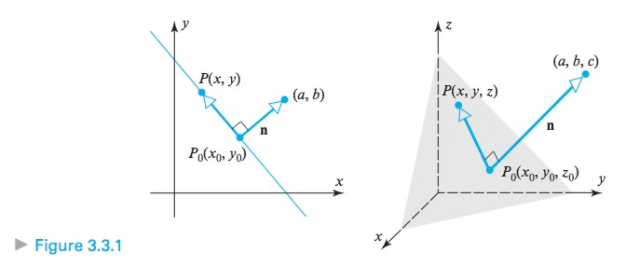
\includegraphics[width=3in]{Images/PointNormal}
\]
The equations and diagram illustrate how a line or plane can be described as the set of points $P$ whose position vector $\overrightarrow{P_0P}$ is orthogonal to a given normal vector $\boldn$. 

The point $P_0$ and vector $\boldn$ determine the line or plane uniquely. 
\end{frame}
\begin{frame}{Example}
Let $\mathcal{P}$ be the plane defined by $\mathcal{P}: 3(x-1)+5(y+2)-7z=0$. 

(a) Describe $\mathcal{P}$ geometrically. 

(b) Give a parametric (or vector) description of the points of $\mathcal{P}$.
\begin{bsolution}
\scriptsize
(a) The normal vector is $\boldn=(3,5,-7)$, and we read off $P_0=(1,-2,0)$ as one point of the plane. The point-normal form then tells us that the plane is the set of all points $P=(x,y,z)$ whose position vector $\overrightarrow{P_0P}$ is orthogonal to $\boldn$. 
\bpause
(b)  Algebraically, the plane is just the set of all solutions $(x,y,z)$ to the given linear equation, which we now write in the standard way:
\[
3x+5y-7z=-7.
\]
Gaussian elimination tells us that $y$ and $z$ are free variables. Set these equal to parameters $s, t$ and solve for $x$ to get the parametric description 
\begin{eqnarray*}
x&=&\frac{1}{3}(-7-5s+7t)\\
y&=&s\\
z&=&t,
\end{eqnarray*}
where $s,t$ are any real numbers. 

In vector notation, we have 
\[
(x,y,z)=(-\frac{7}{3},0,0)+s(-\frac{5}{3},1,0)+t(\frac{7}{3},0,1).
\]
Note that the choice of $s=-2$ and $t=0$ yields the original point $P_0=(1,-2,0)$ 
\end{bsolution}
\end{frame}
\begin{frame}{Vector parametrization of lines and planes}
\alert{Planes}. As the previous example illustrates, any plane $\mathcal{P}$ can be described by a vector parametrization. That is $\mathcal{P}$ is the set of points of the form 
\[
\boldx=\boldx_0+s\boldv_0+t\boldw_0,
\]
where $\boldx_0$ is a fixed point on on the plane, and $\boldv_0$ and $\boldw_0$ are two fixed vectors describing the directions in which the plane ``spreads out". The \alert{two} free parameters $s$ and $t$ are allowed to vary freely, consistent with our idea of a plane as a \alert{2-dimensional} object. 
\bpause
\alert{Lines}. Similarly we can give a vector parametrization of a line as the set of points of the form 
\[
\boldx=\boldx_0+t\boldv_0,
\]
where $\boldx_0$ is a fixed point on the line, $\boldv_0$ is a fixed vector pointing along the line, and $t$ is a free parameter. 
\bpause 
Note the difference between this description and an equation for the plane. 
\bspace
An equation only defines the plane \alert{implicitly} as the set of solutions to an equation, leaving it to you to do the work. 
\bpause 
The vector parametrization gives an \alert{explicit} recipe for writing down different points in the plane. It says to start off at $\boldx_0$ and then add any scalar multiple of $\boldv_0$ and $\boldw_0$ to this. 
\end{frame}
\begin{frame}{Orthogonal projection onto line}
A vector $\boldv$ in $\R^2$ or $\R^3$ determines a line $\ell$: namely, the set of all scalar multiples $c\boldv$ of the vector. 

Given another vector $\boldu$ we call its {\bf orthogonal projection} onto $\boldv$ the vector obtained by ``dropping the perpendicular" from $\boldu$ to the line $\ell$. 
\bpause 
We can clarify this using vector notation. The projection is the vector $\boldw$ along $\ell$ such that the difference vector $\bolde=\boldu-\boldw$ is \alert{orthogonal} to $\ell$.
\bpause
How do we find $\boldw$?  Since it lies along $\ell$ it is of the form $c\boldv$ for some constant $c$. Since we want $\bolde=\boldu-\boldw=\boldu-c\boldv$ to be orthogonal to $\ell$, we need 
\[
(\boldu-c\boldv)\cdot\boldv=0,
\]
or equivalently, 
\[
c(\boldv\cdot\boldv)=\boldu\cdot\boldv.
\]
\pause We conclude $c=\frac{\boldu\cdot\boldv}{\boldv\cdot\boldv}$. 

This gives us a formula for the orthogonal projection of $\boldu$ onto $\boldv$!!
\end{frame}
\begin{frame}{Orthogonal projection onto line}
I restricted the prior discussion to $\R^2$ and $\R^3$ just for the sake of intuition, but the concept and formula extend directly to any $\R^n$. 
\bpause
\alert{Orthogonal projection:} let $\boldu$ and $\boldv$ be any vectors in $\R^n$. The {\bf orthogonal projection} of $\boldu$ onto $\boldv$ is the unique vector $\boldw$ satisfying 
\bb[(i)]
\ii $\boldw=c\boldv$ is a scalar multiple of $\boldv$, 
\ii the difference vector $\bolde=\boldu-\boldw$ is orthogonal to $\boldv$. 
\ee
We denote this vector as $\proj{\boldu}{\boldv}$, and compute it using the following formula:
\[
\proj{\boldu}{\boldv}=c\boldv \ \text{ where  } c=\frac{\boldu\cdot\boldv}{\boldv\cdot\boldv}
\] 
We also call $\proj{\boldu}{\boldv}$ the {\bf vector component of $\boldu$ along $\boldv$}, and the difference vector $\bolde=\boldu-\proj{\boldu}{\boldv}$ the {\bf vector component of $\boldu$ orthogonal to $\boldv$}. 
%\bspace
%The expression $\boldu=\proj_\boldv(\boldu)+\bolde$ gives us a decomposition of $\boldu$ into two orthogonal components. 
\end{frame}
\begin{frame}{Orthogonal projection as ``closest vector"}
We can show that the orthogonal projection $\proj{\boldu}{\boldv}$ is the vector along the line $\ell$ defined by $\boldv$ that is \alert{closest} to $\boldu$: i.e., we have $\norm{\boldu-\proj{\boldu}{\boldv}}\leq\norm{\boldu-\boldw}$, where $\boldw=c\boldv$ is any other vector along $\ell$. 
\bpause
Indeed, let $\boldw=c\boldv$ be any other vector along $\ell$. Decomposing $\boldu=\proj{\boldu}{\boldv}+\bolde$ into its two orthogonal components, we find that 
\begin{eqnarray*}
\norm{\boldu-\boldw}&=&\norm{\proj{\boldu}{\boldv}+\bolde-\boldw}\\
&=&\norm{(\proj{\boldu}{\boldv}-\boldw)+\bolde}\\
&=&\norm{\proj{\boldu}{\boldv}-\boldw}+\norm{\bolde}.
\end{eqnarray*}
\pause The last equality follows from the generalized Pythagorean theorem and the fact that $\bolde$ is orthogonal to $\boldw'=\proj{\boldu}{\boldv}-\boldw$. Why is this last statement true? Because both $\proj{\boldu}{\boldv}$ and $\boldw$ are multiples of $\boldv$, making $\boldw'$ a scalar multiple of $\boldv$; since $\bolde$ is orthogonal to $\boldv$, it is orthogonal to any multiple of $\boldv$! 

\bpause
Finally the equality 
\[
\norm{\boldu-\boldw}=\norm{\proj{\boldu}{\boldv}-\boldw}+\norm{\bolde}
\]
shows that $\norm{\boldu-\boldw}\geq \norm{\bolde}=\norm{\boldu-\proj{\boldu}{\boldv}}$, as desired. 
\end{frame}
\begin{frame}{Projection onto a plane}
Suppose we have a plane $\mathcal{P}: a(x-x_1)+b(y-y_1)+c(z-z_1)=0$, and a point $P_0=(x_0,y_0,z_0)$ in $\R^3$. How do we find the point $P=(x,y,z)$ in the plane closest to $P_0$? 
\bpause Intuition tells us that it should be the point obtained by  ``dropping the perpendicular" from $P_0$ to the plane. 
\[
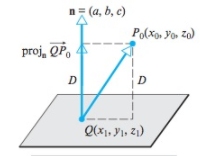
\includegraphics[width=1in]{Images/ProjPlane}
\]
\pause
Assuming this is true (it is, as a proof similar to the one on the last slide shows), how do we find  the point $P$, called the {\bf orthogonal projection of $P_0$ onto the plane}? 
\bpause
As the diagram suggests, letting $Q=(x_1,y_1,z_1)$ we should take the projection of $\boldu=\overrightarrow{QP_0}$ onto the normal vector $\boldn=(a,b,c)$, and subtract this from $P_0$. 
\bspace That is the projection of $P_0$ onto the plane is the point 
\[
P=P_0-\proj{\boldu}{\boldn},
\]
and the distance from $P_0$ to the plane is thus $\norm{\proj{\boldu}{\boldn}}$. 
\end{frame}
\begin{frame}{Example}
Let $\mathcal{P}$ be the plane $(x-1)+(y-1)+2(z-1)=0$, and let $P_0=(0,1,5)$. Find the distance from $P_0$ to the plane. 
\pause
\[
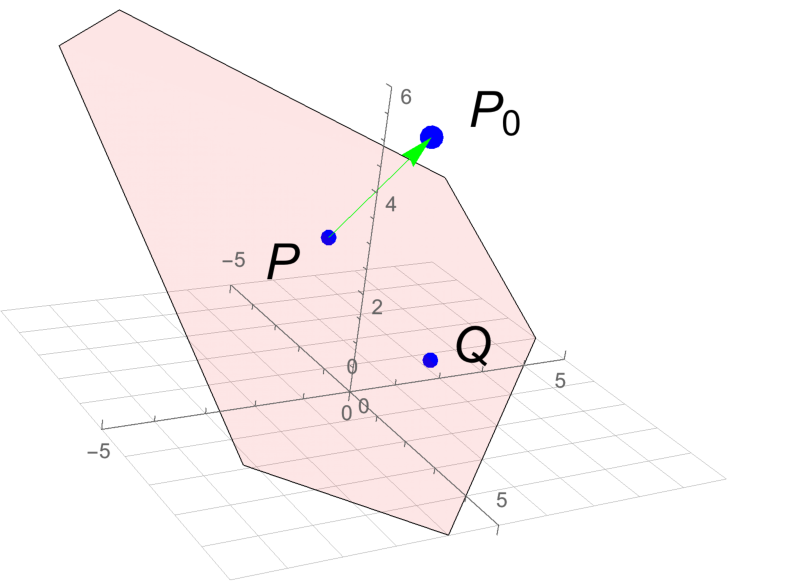
\includegraphics[width=1.5in]{Images/ProjPlaneEx}
\]
Let $Q=(1,1,1)$, a point in the plane. 

The green arrow is the projection of $\boldu=\overrightarrow{QP_0}=(0,1,5)-(1,1,1)=(-1,0,4)$ onto the normal vector $\boldn=(1,1,2)$. 
\bpause
This is computed as $\proj{\boldu}{\boldn}=c\boldn$, where $c=\frac{\boldu\cdot\boldn}{\boldn\cdot\boldn}=\frac{7}{6}$. 

\pause
Thus $\proj{\boldu}{\boldn}=(7/6,7/6,7/3)$. 

The projection of $P_0$ onto the plane is $P=P_0-\proj{\boldu}{\boldn})=(-7/6,-1/6,8/3)$. 

The distance from $P_0$ to the plane is the length of the green vector:$\norm{\proj{\boldu}{\boldn}}=\sqrt{49/36+49/36+49/9}=7\sqrt{6}/6$. 

\end{frame}
